\documentclass[lang=cn]{elegantbook}

%% 引入宏包
\usepackage{tkz-euclide}

%% elegantbook 设置
\renewcommand{\examplename}{题}
\renewcommand{\notename}{分析}
\renewcommand{\solutionname}{解答}
\renewcommand{\theexam}{\arabic{exam}}
\renewenvironment{example}[1][]{
  \refstepcounter{exam}
  \par\noindent\textbf{\color{main}{\examplename} \theexam #1 }\;\rmfamily}{
  \par\ignorespacesafterend}
\renewenvironment{note}{\par\noindent\textbf{\color{second}\notename} \;\citshape}{\par}
\renewenvironment{solution}{\par\noindent\textbf{\color{third}\solutionname} \;}{\par}

%% 行间距
\linespread{1.8}

%% 句号
\catcode`。=\active
\def。{.}

%% 分数
\let\oldfrac=\frac
\let\frac=\dfrac

%% 平行
\renewcommand{\parallel}{\ensuremath{\mathrel{\!/\mkern-5mu/\!}}}
\catcode`∥=\active
\def∥{\parallel}

% 带圈数字
% \renewcommand{\circled}[1]{\raisebox{.5pt}{\textcircled{\raisebox{-.8pt} {\small #1}}}}
\catcode`①=\active
\catcode`②=\active
\catcode`③=\active
\catcode`④=\active
\catcode`⑤=\active
\catcode`⑥=\active
\catcode`⑦=\active
\catcode`⑧=\active
\catcode`⑨=\active
\def①{\circled{1}}
\def②{\circled{2}}
\def③{\circled{3}}
\def④{\circled{4}}
\def⑤{\circled{5}}
\def⑥{\circled{6}}
\def⑦{\circled{7}}
\def⑧{\circled{8}}
\def⑨{\circled{9}}




%% 调整题目编号
\setcounter{exam}{25}

\begin{document}

\chapter*{2022年朝阳一模压轴题分析与解答}

\begin{example}
  在平面直角坐标系$xOy$中,点$\left( -2,0 \right),\left( -1,y_1 \right),\left( 1,y_2 \right),\left( 2,y_3 \right)$在抛物线$y=x^2+bx+c$上.

  (1)若$y_1=y_2$,求$y_3$的值;

  (2)若$y_2<y_1<y_3$,求$y_3$的取值范围.
\end{example}

\begin{note}
  (1)直接根据二次函数图象的对称性,得出二次函数的对称轴为$x=0$,于是可以求出$y_3$的值。
  
  (2)首先带入$\left( -2,0 \right)$点,可以得出$b$、$c$之间的关系,消去参数$c$。于是$y_3$可以用$b$表示出来。因此我们只需要求出$b$的取值范围就可以了。
  
  思路1:根据$y_2<y_1<y_3$的条件,判断对称轴$x=-\frac{b}{2}$的位置;
  
  思路2:直接带入横坐标,求出$y_1$、$y_2$、$y_3$的值,解出$b$的取值范围。
\end{note}

\begin{solution}
  (1)由$y_1=y_2$可知,抛物线的对称轴为$y$轴,而$\left( -2,0 \right)$和$\left( 2,y_3 \right)$关于$y$轴对称,所以$y_3=0$。
  
  (2)把$\left( -2,0 \right)$带入抛物线的解析式,得$0=\left( -2 \right)^2-2b+c$,$\therefore c=2b-4$,$y=x^2+bx+2b-4$。
  
  分别把$(-1,y_1)$、$(1,y_2)$、$(2,y_3)$带入抛物线的解析式,可得$y_1=b-3$,$y_2=3b-3$,$y_3=4b$。
  
  $\because y_2<y_1<y_3$,$\therefore 3b-3<b-3<4b$,解得$-1<b<0$。
  
  因此$-4<y_3<0$。
\end{solution}

\newpage


\begin{example}
  在$\triangle ABC$中,$D$是$BC$的中点,且$\angle BAD\ne 90{}^\circ$,将线段$AB$沿$AD$所在直线翻折,得到线段$AB'$,作$CE\parallel AB$交直线$AB'$于点$E$.
  
  (1)如图,若$AB>AC$,
  
  ①\,依题意补全图形;
  
  ②\,用等式表示线段$AB$,$AE$,$CE$之间的数量关系,并证明;
  
  (2)若$AB<AC$,上述结论是否仍然成立?若成立,简述理由;若不成立,直接用等式表示线段$AB$,$AE$,$CE$之间新的数量关系(不需证明).

  \hfill\begin{tikzpicture}[semithick]
  \tkzDefPoints{0/0/B, 3/0/C}
  \tkzDefMidPoint(B,C) \tkzGetPoint{D}
  \tkzDefShiftPoint[D](48:2.8){A}
  
  \tkzDrawPolygon[](A,B,C)
  \tkzDrawSegment[line join=bevel](A,D)
  
  \tkzLabelPoints[above=-1.5pt](A)
  \tkzLabelPoints[below left=-3pt](B)
  \tkzLabelPoints[below right=-3pt](C)
  \tkzLabelPoints[below=-1.5pt](D)
  
\end{tikzpicture}
\end{example}

\begin{note}
  (1)①\,直接根据题目要求画出图象即可。

  ②\,由对称性可知,$AB=AB'$,因此问题可以转换成求$AB'$,$AE$,$CE$之间的数量关系。由图象可知,$AB'-AE=B'E$,因此只需要找出$B'E$和$CE$之间的关系即可。根据图象,可以猜测:$B'E=CE$。

  要证明$B'E=CE$,只需要连接$CB'$,证明$\angle ECB=\angle EB'C$即可。

  由中点和对称的条件可知,$DC=DB=DB'$,$\therefore \angle DCB'=\angle DB'C$,因此只需要证明$\angle DCE=\angle DB'E$。

  由平行和对称的条件可知,$\angle DCE=\angle B=\angle DB'E$,命题得证。

  (3)画出图象,类似(2)中的方法,把$AB$和$AE$转换为$B'E$,再由$B'E=CE$即可得出结论。

  {\color{red!80!black} 需要注意的是,题目中有一个$\angle BAD\ne 90^\circ$的条件,看似没有用处,实际上这个条件保证了直线$AB'$与过$C$点的平行线一定有交点。
  
  另外,这个条件还提示我们,要去画一下$\angle BAD<90^\circ$和$\angle BAD>90^\circ$两种情况,这两种情况下,$A$、$B'$、$E$三个点位置关系不一样,因此得出的结论也不一样。}
\end{note}

\begin{solution}
  (1)① 如图1:

  \begin{center}
    \begin{tabular}{ccc}
      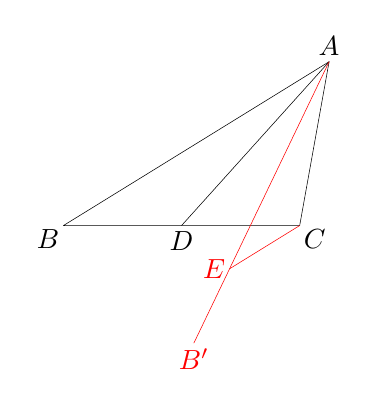
\begin{tikzpicture}[semithick]
  \tkzDefPoints{0/0/B, 3/0/C}
  \tkzDefMidPoint(B,C) \tkzGetPoint{D}
  \tkzDefShiftPoint[D](48:2.8){A}
  
  \tkzDrawPolygon[](A,B,C)
  \tkzDrawSegment[line join=bevel](A,D)
  
  \tkzLabelPoints[above=-1.5pt](A)
  \tkzLabelPoints[below left=-3pt](B)
  \tkzLabelPoints[below right=-3pt](C)
  \tkzLabelPoints[below=-1.5pt](D)
  
  \tkzDefPointBy[reflection=over A--D](B) \tkzGetPoint{B'}
  \tkzDefLine[parallel=through C](A,B)
  \tkzInterLL(A,B')(C,tkzPointResult) \tkzGetPoint{E}
  
  \tkzDrawSegments[red](A,B' C,E)
  
  \tkzLabelPoints[red,below=-1.5pt](B')
  \tkzLabelPoints[red,left=-2pt](E)
  
\end{tikzpicture} & \hspace*{10mm} & 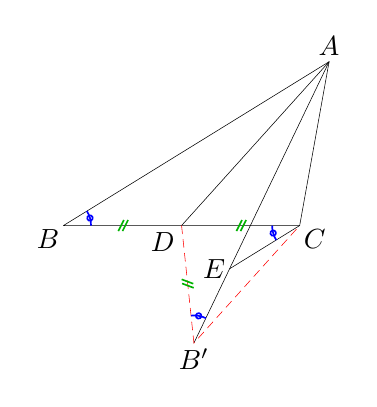
\begin{tikzpicture}[semithick]
  \tkzDefPoints{0/0/B, 3/0/C}
  \tkzDefMidPoint(B,C) \tkzGetPoint{D}
  \tkzDefShiftPoint[D](48:2.8){A}
  
  \tkzDrawPolygon[](A,B,C)
  \tkzDrawSegment[line join=bevel](A,D)
  
  \tkzLabelPoints[above=-1.5pt](A)
  \tkzLabelPoints[below left=-3pt](B)
  \tkzLabelPoints[below right=-3pt](C)
  \tkzLabelPoints[below left=-1.5pt](D)
  
  \tkzDefPointBy[reflection=over A--D](B) \tkzGetPoint{B'}
  \tkzDefLine[parallel=through C](A,B)
  \tkzInterLL(A,B')(C,tkzPointResult) \tkzGetPoint{E}
  
  \tkzDrawSegments[](A,B' C,E)
  
  \tkzLabelPoints[below=-1.5pt](B')
  \tkzLabelPoints[left=-2pt](E)
  
  \tkzDrawPolySeg[red, densely dashed](D,B',C)
  \tkzMarkSegments[mark=s||, color=green!70!black, size=2pt](B,D D,C B',D)
  \tkzMarkAngles[size=.35, color=blue, mark=o, mksize=1pt, mkcolor=blue](E,B',D B,C,E C,B,A)
\end{tikzpicture} \\[-1ex]
      图1 & & 图2
    \end{tabular}
  \end{center}

  ② $AB-AE=CE$。
  
  如图2,连接$B'D$、$B'C$。
  
  由对称性可知$AB=AB'$,$\triangle ABD\cong \triangle AB'D$,
  
  $\therefore BD=B'D$,$\angle B=\angle DB'E$。
  
  $\because BD=CD$,
  $\therefore B'D=CD$,
  $\therefore \angle DCB'=\angle DB'C$。
  
  $\because CE\parallel AB$,
  $\therefore \angle DCE=\angle B$,
  $\therefore \angle DCE=\angle DB'E$。
  
  $\therefore \angle ECB'=\angle DCB'-\angle ECB'=\angle DB'C-\angle DB'E=\angle DB'C$,
  
  $\therefore CE=B'E=AB'-AE=AB-AE$。

  (3)如图3,当$\angle BAD<90^\circ$时,$AE-AB=CE$;
  
  如图4,当$\angle BAD>90^\circ$时,$AE+AB=CE$。

  \begin{center}
    \begin{tabular}{ccc}
      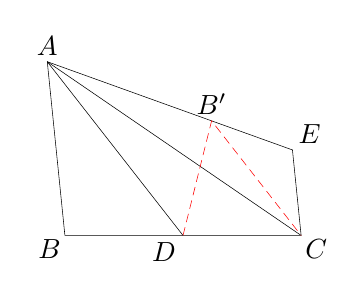
\begin{tikzpicture}[semithick]
  \tkzDefPoints{0/0/B, 3/0/C}
  \tkzDefMidPoint(B,C) \tkzGetPoint{D}
  \tkzDefShiftPoint[D](128:2.8){A}
  
  \tkzDrawPolygon[](A,B,C)
  \tkzDrawSegment[line join=bevel](A,D)
  
  \tkzLabelPoints[above=-1.5pt](A)
  \tkzLabelPoints[below left=-3pt](B)
  \tkzLabelPoints[below right=-3pt](C)
  \tkzLabelPoints[below left=-1.5pt](D)
  
  \tkzDefPointBy[reflection=over A--D](B) \tkzGetPoint{B'}
  \tkzDefLine[parallel=through C](A,B)
  \tkzInterLL(A,B')(C,tkzPointResult) \tkzGetPoint{E}
  
  \tkzDrawSegments[](A,E C,E)
  
  \tkzLabelPoints[above=-1.5pt](B')
  \tkzLabelPoints[above right=-2pt](E)
  
  \tkzDrawPolySeg[red, densely dashed](D,B',C)
%   \tkzMarkSegments[mark=s||, color=green!70!black, size=2pt](B,D D,C B',D)
%   \tkzMarkAngles[size=.35, color=blue, mark=|, mksize=1pt, mkcolor=blue](A,B',D C,B,A)
%   \tkzMarkAngles[size=.2, color=cyan, mark=o, mksize=1.5pt, mkcolor=cyan](E,C,D D,B',E)
\end{tikzpicture} & \hspace*{10mm} & 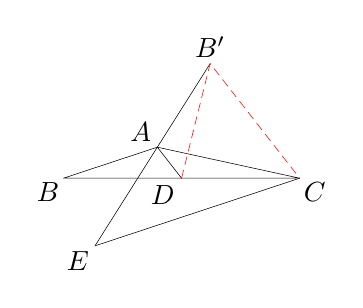
\begin{tikzpicture}[semithick]
  \tkzDefPoints{0/0/B, 3/0/C}
  \tkzDefMidPoint(B,C) \tkzGetPoint{D}
  \tkzDefShiftPoint[D](128:0.5){A}
  
  \tkzDrawPolygon[](A,B,C)
  \tkzDrawSegment[line join=bevel](A,D)
  
  \tkzLabelPoints[above left=-2pt](A)
  \tkzLabelPoints[below left=-3pt](B)
  \tkzLabelPoints[below right=-3pt](C)
  \tkzLabelPoints[below left=-1.5pt](D)
  
  \tkzDefPointBy[reflection=over A--D](B) \tkzGetPoint{B'}
  \tkzDefLine[parallel=through C](A,B)
  \tkzInterLL(A,B')(C,tkzPointResult) \tkzGetPoint{E}
  
  \tkzDrawSegments[](B',E C,E)
  
  \tkzLabelPoints[above=-1.5pt](B')
  \tkzLabelPoints[below left=-2pt](E)
  
  \tkzDrawPolySeg[red, densely dashed](D,B',C)
%   \tkzMarkSegments[mark=s||, color=green!70!black, size=2pt](B,D D,C B',D)
%   \tkzMarkAngles[size=.65, color=blue, mark=o, mksize=1pt, mkcolor=blue](E,B',D B,C,E C,B,A)
\end{tikzpicture} \\[-1ex]
      图3 & & 图4
    \end{tabular}
  \end{center}
\end{solution}

\newpage



\begin{example}
  在平面直角坐标系$xOy$中,对于直线$l:y=kx+b$,给出如下定义:若直线$l$与某个圆相交,则两个交点之间的距离称为直线$l$关于该圆的“圆截距”.
  
  (1)如图1,$\odot O$的半径为1,当$k=1,b=1$时,直接写出直线$l$关于$\odot O$的“圆截距”;
  
  (2)点$M$的坐标为$\left( 1,0 \right)$,
  
  ①\,如图2,若$\odot M$的半径为1,当$b=1$时,直线$l$关于$\odot M$的“圆截距”小于$\frac{4}{5}\sqrt{5}$,求$k$的取值范围;
  
  ②\,如图3,若$\odot M$的半径为2,当$k$的取值在实数范围内变化时,直线$l$关于$\odot M$的“圆截距”的最小值2,直接写出$b$的值.

  \begin{center}
    \begin{tabular}{ccc}
      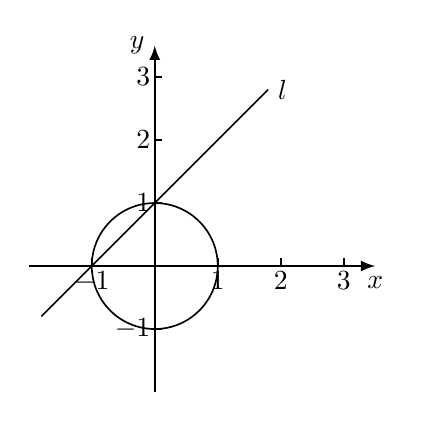
\begin{tikzpicture}[>=latex, semithick, scale=.8]
  \draw[->, thick] (-2,0) -- (3.5,0) node[below] {$x$};
  \draw[->, thick] (0,-2) -- (0,3.5) node[left] {$y$};
  \foreach \i in {-1,1,2,3} {
    \draw (\i,0) node[below=-1.5pt] {$\i$} -- (\i, 0.12);
    \draw (0,\i) node[left=-2pt] {$\i$} -- (0.12,\i);
  }
  \draw (0,0) circle (1cm);
  \draw[smooth, domain=-1.8:1.8] plot (\x, \x+1) node[right] {$l$};
\end{tikzpicture} & 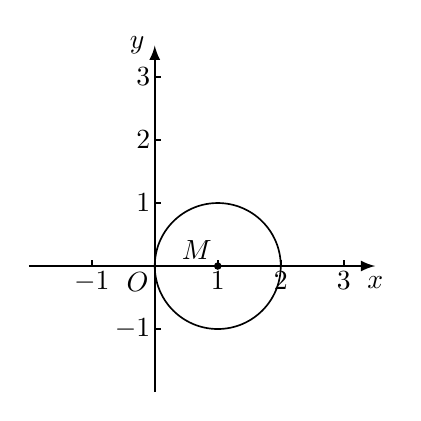
\begin{tikzpicture}[>=latex, semithick, scale=.8]
  \draw[->, thick] (-2,0) -- (3.5,0) node[below] {$x$};
  \draw[->, thick] (0,-2) -- (0,3.5) node[left] {$y$};
  \path (0,0) node[below left=-2pt] {$O$};
  \foreach \i in {-1,1,2,3} {
    \draw (\i,0) node[below=-1.5pt] {$\i$} -- (\i, 0.1);
    \draw (0,\i) node[left=-2pt] {$\i$} -- (0.1,\i);
  }
  \draw[fill] (1,0) node[above left=-2pt] {$M$} circle (1.3pt);
  \draw (1,0) circle (1cm);
%   \draw[smooth, domain=-1.8:1.8] plot (\x, \x+1) node[right] {$l$};
\end{tikzpicture} & 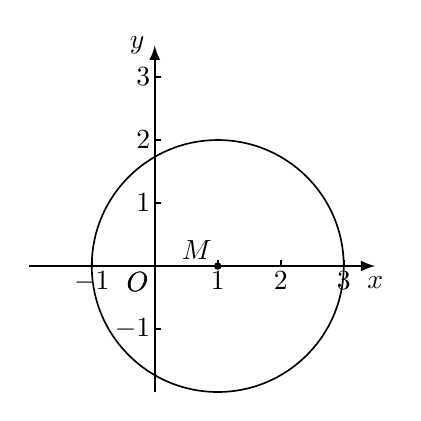
\begin{tikzpicture}[>=latex, semithick, scale=.8]
  \draw[->, thick] (-2,0) -- (3.5,0) node[below] {$x$};
  \draw[->, thick] (0,-2) -- (0,3.5) node[left] {$y$};
  \path (0,0) node[below left=-2pt] {$O$};
  \path (0,0) node[below left=-2pt] {$O$};
  \foreach \i in {-1,1,2,3} {
    \draw (\i,0) node[below=-1.5pt] {$\i$} -- (\i, 0.1);
    \draw (0,\i) node[left=-2pt] {$\i$} -- (0.1,\i);
  }
  \draw[fill] (1,0) node[above left=-2pt] {$M$} circle (1.3pt);
  \draw (1,0) circle (2cm);
%   \draw[smooth, domain=-1.8:1.8] plot (\x, \x+1) node[right] {$l$};
\end{tikzpicture} \\[-1ex]
      图1 & 图2 & 图3
    \end{tabular}
  \end{center}
\end{example}

\begin{note}
  对于新定义类型的题目,我们首先要分析清楚它给的定义,最好能够把“新”定义转换为我们熟悉的定义。

  这道题中,所谓的“圆截距”,其实就是直线与圆相交时的弦长。根据垂径定理,我们可以得出弦长公式:
  $$
    \text{弦长}=2\sqrt{r^2-d^2}
  $$
  其中$r$为圆的半径,$d$为弦心距。

  因此,涉及弦长的问题,可以转换为关于圆心与直线之间的距离的问题。

  (1)有图象可知,两个交点为$(-1,0)$和$(0,1)$,则弦长为$\sqrt{2}$。

  (2)当“圆截距”恰好为$\frac{4}{5}\sqrt{5}$时,由弦长公式$2\sqrt{1^2-d^2}=\frac{4}{5}\sqrt{5}$,可得$d=\frac{\sqrt{5}}{5}$。如果知道点到直线距离公式的话,可以直接求出此时直线$l$的斜率:$d=\frac{\left|k+1\right|}{\sqrt{k^2+1}}=\frac{\sqrt{5}}{5}$,解得$k=-\frac{1}{2}$或$k=-2$。
 
  如果不知道点到直线的距离公式的话,我们据需要观察此时弦在圆中的位置。如图4,在$\odot M$中,$MA=MB=1$,$AB=\frac{4}{5}\sqrt{5}$,由上面的计算可知,$MN=\frac{1}{5}\sqrt{5}$,$NB=\frac{2}{5}\sqrt{5}$,因此$\tan \angle ABM=\frac{1}{2}$是一个定值。

  观察图5,设$l$与$y$轴的交点为$P(0,1)$。如果取$B(2,0)$,则$\tan \angle PBM=\frac{1}{2}$恰好满足条件,此时$k_{PB}=-\frac{1}{2}$。
  
  \begin{center}
    \begin{tabular}{ccc}
      \begin{tikzpicture}[semithick, scale=1.2]
  \tkzDefPoint(0,0){M}
  \pgfmathsetmacro\r{\fpeval{1/sqrt(5)}}
  \tkzDefPointOnCircle[R=angle 70 center M radius \r] \tkzGetPoint{N}
  \tkzDefTangent[at=N](M)
  \tkzInterLC[R](N,tkzPointResult)(M,1) \tkzGetPoints{B}{A}

  \tkzDrawPoint[size=2](M)
  \tkzDrawCircle[R](M,1)
  \tkzDrawSegments(A,B M,A M,B M,N)

  \tkzLabelPoints[below=-1.5pt](M)
  \tkzLabelPoints[above left=-2pt](A)
  \tkzLabelPoints[right=-1.5pt](B)
  \tkzLabelPoints[above right=-2pt](N)

  \tkzMarkRightAngle[size=.1](M,N,B)
\end{tikzpicture} & 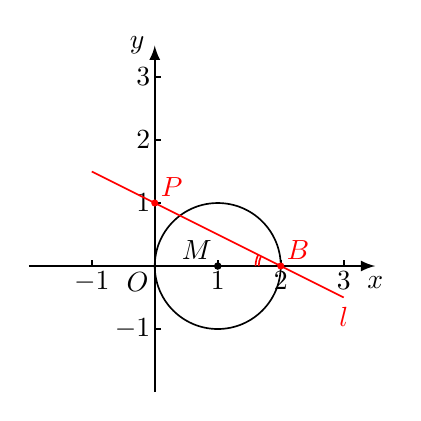
\begin{tikzpicture}[>=latex, semithick, scale=.8]
  \draw[->, thick] (-2,0) -- (3.5,0) node[below] {$x$};
  \draw[->, thick] (0,-2) -- (0,3.5) node[left] {$y$};
  \path (0,0) node[below left=-2pt] {$O$};
  \foreach \i in {-1,1,2,3} {
    \draw (\i,0) node[below=-1.5pt] {$\i$} -- (\i, 0.1);
    \draw (0,\i) node[left=-2pt] {$\i$} -- (0.1,\i);
  }
  \draw[fill] (1,0) node[above left=-2pt] {$M$} circle (1.3pt);
  \draw (1,0) circle (1cm);
  \draw[red, smooth, domain=-1:3] plot (\x, -\x/2+1) node[below] {$l$};
  \draw[red, fill] (0,1) node[above right=-2pt] {$P$} circle (1.2pt);
  \draw[red, fill] (2,0) node[above right=-2pt] {$B$} circle (1.2pt);
  \pgfmathparse{180-atan(0.5)}
  \let\aPB=\pgfmathresult
  \draw[red] (2-0.4,0) arc (180:\aPB:0.4);
  \draw[red] (2-0.35,0) arc (180:\aPB:0.35);
\end{tikzpicture} & 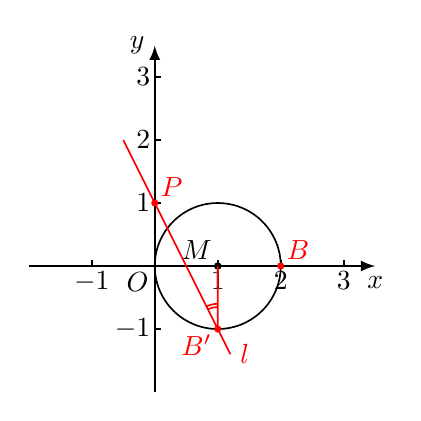
\begin{tikzpicture}[>=latex, semithick, scale=.8]
  \draw[->, thick] (-2,0) -- (3.5,0) node[below] {$x$};
  \draw[->, thick] (0,-2) -- (0,3.5) node[left] {$y$};
  \path (0,0) node[below left=-2pt] {$O$};
  \foreach \i in {-1,1,2,3} {
    \draw (\i,0) node[below=-1.5pt] {$\i$} -- (\i, 0.1);
    \draw (0,\i) node[left=-2pt] {$\i$} -- (0.1,\i);
  }
  \draw[fill] (1,0) node[above left=-2pt] {$M$} circle (1.3pt);
  \draw (1,0) circle (1cm);
  \draw[red, smooth, domain=-0.5:1.2] plot (\x, -\x*2+1) node[right] {$l$};
  \draw[red, fill] (0,1) node[above right=-2pt] {$P$} circle (1.2pt);
  \draw[red, fill] (2,0) node[above right=-2pt] {$B$} circle (1.2pt);
  \draw[red, fill] (1,0) -- (1,-1) node[below left=-2pt] {$B'$} circle (1.2pt);
  \pgfmathparse{90+atan(0.5)}
  \let\aPB=\pgfmathresult
  \draw[red] (1,-1+0.4) arc (90:\aPB:0.4);
  \draw[red] (1,-1+0.35) arc (90:\aPB:0.35);
\end{tikzpicture} \\[-1ex]
      图4 & 图5 & 图6
    \end{tabular}
  \end{center}

  由圆的对称性可以知道,如图6,$PB$关于$PM$的对称直线$PB'$也满足条件,此时$B'$为$B$关于$PM$的对称点,坐标为$(1,-1)$,因此$k_{PB'}=-2$。

  求出两个边界条件之后,再根据图象,求出直线与$\odot M$相交,且弦长小于$\frac{4}{5}\sqrt{5}$的情况即可。

  (3)设$l$与$y$轴的交点为$P(0,b)$。若点$P$在$\odot M$上或在$\odot M$外,则“圆截距”没有最小值。因为直线$l$可以与$\odot M$相交,但是无限接近于相切的情况,此时弦长可以无限接近于$0$。

  所以,点$P$一定在圆内。

  那么这个问题就转换为:经过$\odot M$内一点$P$的所用弦中,最短的弦的长度为$2$。

  我们知道,如果$\odot M$与点$P$固定,那么当弦与$MP$垂直的时候,弦长取得最小值,此时弦心距即为$MP$,如图7。
    
  \begin{center}
      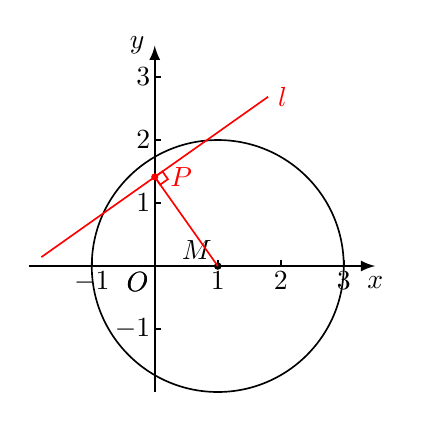
\begin{tikzpicture}[>=latex, semithick, scale=.8]
  \draw[->, thick] (-2,0) -- (3.5,0) node[below] {$x$};
  \draw[->, thick] (0,-2) -- (0,3.5) node[left] {$y$};
  \path (0,0) node[below left=-2pt] {$O$};
  \path (0,0) node[below left=-2pt] {$O$};
  \foreach \i in {-1,1,2,3} {
    \draw (\i,0) node[below=-1.5pt] {$\i$} -- (\i, 0.1);
    \draw (0,\i) node[left=-2pt] {$\i$} -- (0.1,\i);
  }
  \draw[fill] (1,0) node[above left=-2pt] {$M$} circle (1.3pt);
  \draw (1,0) circle (2cm);

  \draw[red, fill] (1,0) -- (0,{sqrt(2)}) node[right=2pt] {$P$} circle (1.2pt);
  \draw[red, smooth, domain=-1.8:1.8] plot (\x, {\x/sqrt(2)+sqrt(2)}) node[right] {$l$};
  \pgfmathparse{atan(1/sqrt(2)}
  \let\k=\pgfmathresult
  \draw[red] (0,{sqrt(2)}) -- ++ (\k:.15) -- ++ ({\k-90}:.15) -- ++({\k+180}:.15) -- cycle;
\end{tikzpicture}\\
      图7
  \end{center}

  此时弦长为$2\sqrt{2^2-MP^2}=2$,解得$MP=\sqrt{3}$。
  
  又知道$M(1,0)$,$P(0,b)$,因此$MP=\sqrt{1^2+b^2}$,解得$b=\pm \sqrt{2}$。
\end{note}

\begin{solution}
  (1)$\sqrt{2}$。

  (2)如图8,当直线讲过点$P(0,1)$,与$\odot M$相交于$A$、$B(2,0)$时,$PB=2\sqrt{5}$,  
  $\therefore \cos \angle PBM=\frac{OB}{PB}=\frac{2}{5}\sqrt{5}$。
  
  过$M$作$MN\perp AB$于$N$,则$N$为$AB$的中点。
  $\therefore AB=2NB=2MB\cos \angle PBM=\frac{4}{5}\sqrt{5}$,因此直线$l$关于$\odot M$的“圆截距”恰好等于$\frac{4}{5}\sqrt{5}$。  
  此时$k=-\frac{1}{2}$。

  \begin{center}
    \begin{tabular}{ccc}
      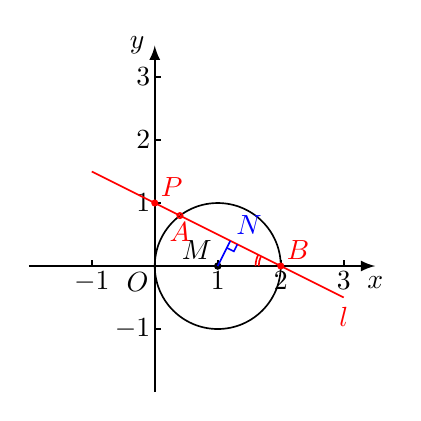
\begin{tikzpicture}[>=latex, semithick, scale=.8]
  \draw[->, thick] (-2,0) -- (3.5,0) node[below] {$x$};
  \draw[->, thick] (0,-2) -- (0,3.5) node[left] {$y$};
  \path (0,0) node[below left=-2pt] {$O$};
  \foreach \i in {-1,1,2,3} {
    \draw (\i,0) node[below=-1.5pt] {$\i$} -- (\i, 0.1);
    \draw (0,\i) node[left=-2pt] {$\i$} -- (0.1,\i);
  }
  \draw[fill] (1,0) node[above left=-2pt] {$M$} circle (1.3pt);
  \draw[name path=circleM] (1,0) coordinate (M) circle (1cm);
  \draw[red, smooth, domain=-1:3, name path=lineL] plot (\x, -\x/2+1) node[below] {$l$};
  \draw[red, fill] (0,1) coordinate (P) node[above right=-2pt] {$P$} circle (1.2pt);
  \draw[red, fill] (2,0) coordinate (B) node[above right=-2pt] {$B$} circle (1.2pt);
  \pgfmathparse{180-atan(0.5)}
  \let\aPB=\pgfmathresult
  \draw[red] (2-0.4,0) arc (180:\aPB:0.4);
  \draw[red] (2-0.35,0) arc (180:\aPB:0.35);
  \draw[red, name intersections={of=circleM and lineL}](intersection-2) coordinate (A) node[below=-1pt] {$A$} circle (1.2pt);
  \draw[blue] (M) -- ($(P)!(M)!(B)$) coordinate (N) node[above right=-2pt] {$N$};
  \draw pic [draw, angle radius=.1cm, blue] {right angle=M--N--B};
\end{tikzpicture} & \hspace*{10mm} & 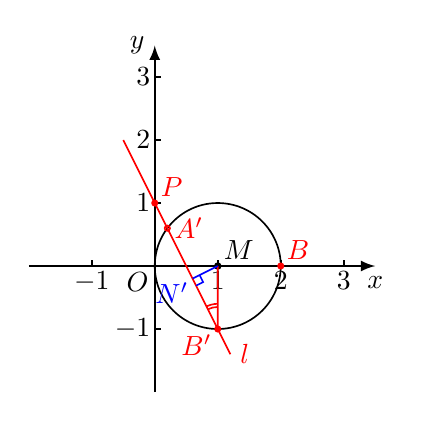
\begin{tikzpicture}[>=latex, semithick, scale=.8]
  \draw[->, thick] (-2,0) -- (3.5,0) node[below] {$x$};
  \draw[->, thick] (0,-2) -- (0,3.5) node[left] {$y$};
  \path (0,0) node[below left=-2pt] {$O$};
  \foreach \i in {-1,1,2,3} {
    \draw (\i,0) node[below=-1.5pt] {$\i$} -- (\i, 0.1);
    \draw (0,\i) node[left=-2pt] {$\i$} -- (0.1,\i);
  }
  \draw[fill] (1,0) node[above right=-2pt] {$M$} circle (1.3pt);
  \draw[name path=circleM] (1,0) coordinate (M) circle (1cm);
  \draw[red, smooth, domain=-0.5:1.2, name path=lineL] plot (\x, -\x*2+1) node[right] {$l$};
  \draw[red, fill] (0,1) coordinate (P) node[above right=-2pt] {$P$} circle (1.2pt);
  \draw[red, fill] (2,0) coordinate (B) node[above right=-2pt] {$B$} circle (1.2pt);
  \draw[red, fill] (1,0) -- (1,-1) coordinate (B') node[below left=-2pt] {$B'$} circle (1.2pt);
  \pgfmathparse{90+atan(0.5)}
  \let\aPB=\pgfmathresult
  \draw[red] (1,-1+0.4) arc (90:\aPB:0.4);
  \draw[red] (1,-1+0.35) arc (90:\aPB:0.35);
  \draw[red, name intersections={of=circleM and lineL}](intersection-1) coordinate (A') node[right=-1pt] {$A'$} circle (1.2pt);
  \draw[blue] (M) -- ($(P)!(M)!(B')$) coordinate (N') node[below left=-3pt] {$N'$};
  \draw pic [draw, angle radius=.1cm, blue] {right angle=M--N'--B'};
\end{tikzpicture} \\[-1ex]
      图8 &  & 图9
    \end{tabular}
  \end{center}

  同理,如图9,当直线经过点$B'(1,-1)$时,直线$l$关于$\odot M$的“圆截距”也恰好等于$\frac{4}{5}\sqrt{5}$。此时$k=-2$。

  结合图象可知,$k$的取值范围为$k<-2$或$-\frac{1}{2}<k<0$。

  (3)$b=\pm\sqrt{2}$。
\end{solution}

\end{document}